\subsection{Geometry preparation}
\label{subsec:geometry_preparation}

The first step in the CFD simulation is to prepare the geometry of the model rocket and import it into \texttt{DesignModeler} of \texttt{Ansys Fluent}.

Once the main geometry is imported, we need to create the computational domain around the rocket.
For this study, we opted for a simple rectangular domain, with a length of $1.5m$ ($0.5m$ in front of the rocket and $1m$ behind it) and a height and width of $0.7m$ (see Figure \ref{fig:rocket_geometry}).

\begin{figure}[H]
    \centering
    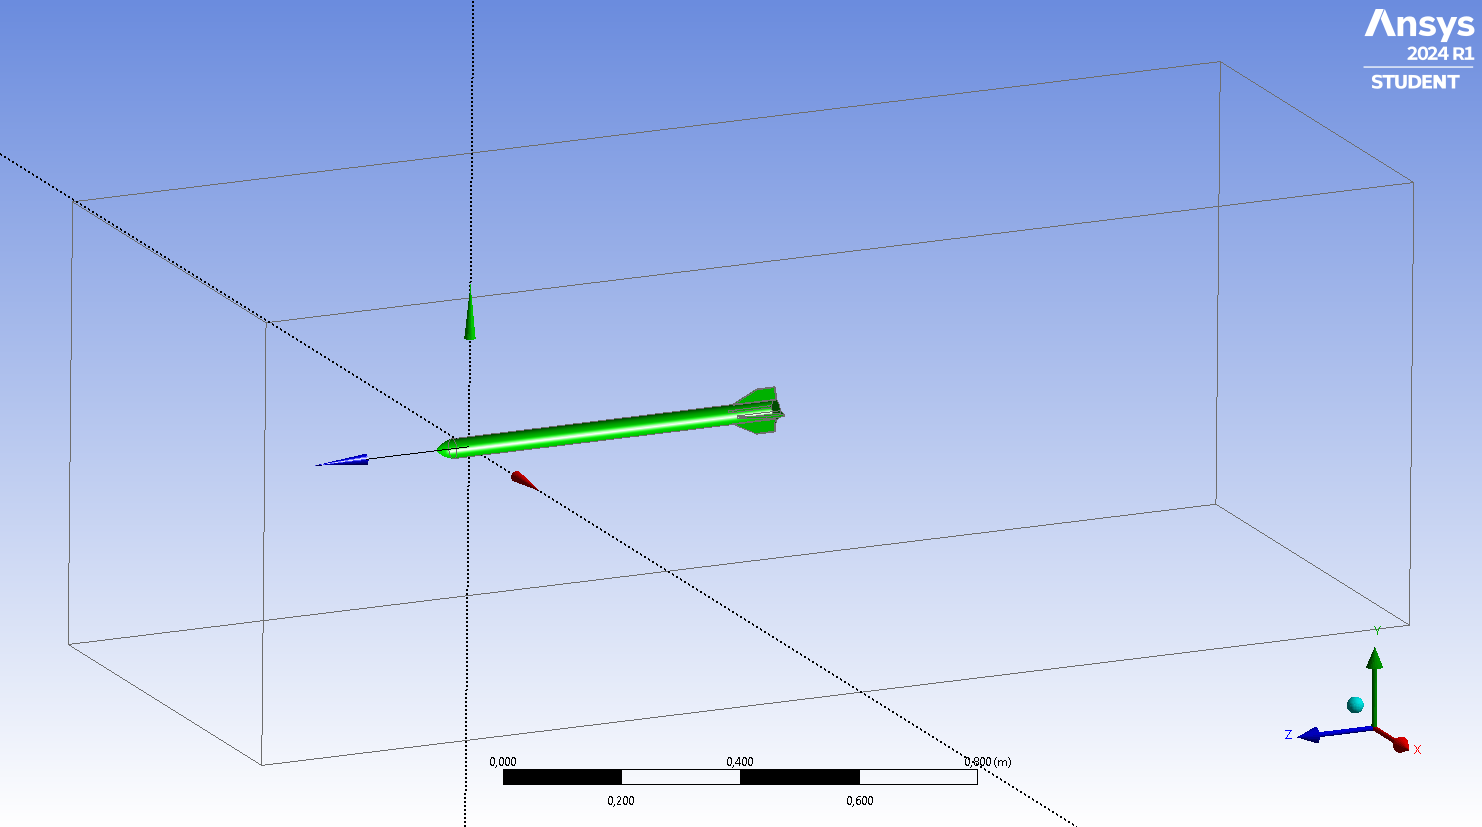
\includegraphics[width=.7\textwidth]{img/DesignModeler.png}
    \caption{Geometry of the model rocket and the surrounding domain in \texttt{DesignModeler}.}
    \label{fig:rocket_geometry}
\end{figure}

The choice in the size of the domain was driven by the idea of having enough space around the rocket to allow the flow to develop and avoid any boundary effects that could affect the results.
In fact, the domain distance in the radial direction from the rocket is about 10 times ($0.7/2 = 0.35 \approx 0.34 = 10 * 0.034$) the diameter of the rocket, which is a common rule of thumb for the size of the domain in CFD simulations.
